
\section{\LSEQ : une fonction d'allocation polylogarithmique}
\label{repl:sec:proposal}

\LSEQ (\emph{polyLogarithmic SEQuence}) est une fonction d'allocation
d'identifiants de taille variable. L'algorithme~\ref{repl:algo:allocpath} montre
les instructions de \LSEQ : la fonction \textsc{allocPath} choisit le chemin
associé à chaque élément afin d'encoder sa position relative à l'égard de ses
éléments adjacents dans la séquence. Dans le but de conserver de bonnes
performances, la profondeur de l'arbre doit rester aussi petite que possible.

\begin{algorithm}
  
\begin{algorithmic}[1]

\small
\algrenewcommand{\algorithmiccomment}[1]{\hskip2em$\rhd$ #1}
\newcommand*{\comment}[1]{$\rhd$ #1}

  \State \textbf{let} $boundary \leftarrow 10$; \hfill \comment{Any constant} 
  \State \textbf{let} $h:\mathbb{N} \rightarrow (\mathcal{P}\times
  \mathcal{P}\rightarrow \mathcal{P})$; \hfill \comment{Get sub-allocation
    function}
  \Statex
    \Function{allocPath}{$p,\, q \in \mathcal{P}$}
    $\rightarrow \mathcal{P}$
    \State \textbf{let} $\langle depth,\,\_ \rangle 
    \leftarrow \textsc{getDepthInterval}(p,\,q)$;
    \State \textbf{return} $h(depth)(p,\,q)$; 
    \hfill \comment{Defers the call to a sub-allocation function}
    \EndFunction
    \Statex
    \Function{left-to-right}{$p,\,q \in \mathcal{P}$}\label{line:lefttoright}
    $\rightarrow \mathcal{P}$
    \State \textbf{let} 
    $\langle depth,\,interval \rangle \leftarrow \textsc{getDepthInterval}(p,\,q);$
    \hfill \comment{\#1 Get the depth of the new path}
    \State \textbf{let} $step \leftarrow min(boundary,\,interval)$;
    \hfill \comment{\#2 Maximal space between two identifiers}
    \State \textbf{return} $\textsc{subPath}(p,\,depth) + rand(0,\,step)$;
    \hfill \comment{\#3 Create the new path}
    \EndFunction
    \Statex
    \Function{right-to-left}{$p,\,q \in \mathcal{P}$}\label{line:righttoleft}
    $\rightarrow \mathcal{P}$
    \State \textbf{let}
    $\langle depth,\, interval\rangle \leftarrow \textsc{getDepthInterval}(p,\,q);$
    \hfill \comment{\#1}
    \State \textbf{let} $step \leftarrow min(boundary,\,interval)$;
    \hfill \comment{\#2}
    \State \textbf{return} $\textsc{subPath}(q,\,depth) - rand(0,\,step)$;
    \hfill \comment{\#3}
    \EndFunction
    \Statex 
    \Function{getDepthInterval}{$p,\,q \in \mathcal{P}$} $\rightarrow \mathbb{N} \times \mathbb{N}$ \hfill \comment{Enough space for 1 path?}
      \State \textbf{let} $depth \leftarrow 0$; $interval \leftarrow 0$;
      \While{$(interval < 2)$}
        \State $depth \leftarrow depth + 1$;
        \State $interval \leftarrow \textsc{subPath}(q,\,depth) - \textsc{subPath}(p,\,depth)$;
      \EndWhile
      \State \textbf{return} $\langle depth,\, interval\rangle$;
    \EndFunction

  \end{algorithmic}


  \caption[Allocation des chemins selon \LSEQ]
  {\label{repl:algo:allocpath}Allocation des chemins selon \LSEQ.}
\end{algorithm}

La fonction \textsc{allocPath} calcule la distance entre les deux chemins
adjacents. L'objectif est de trouver le plus petit niveau de l'arbre exponentiel
(cf. §\ref{repl:subsec:exponentialtree}) contenant assez d'espace pour
accueillir le nouvel élément.  Ensuite, une fonction de hachage $h$
(cf. §\ref{repl:subsec:allocationchoice}) défère l'allocation du chemin à une
sous-fonction d'allocation (cf. §\ref{repl:subsec:suballocation}) selon la
profondeur trouvée.  La sous-fonction d'allocation calcule alors l'intervalle à
disposition et la profondeur du nouveau chemin. Si l'intervalle est plus grand
que la limite imposée, alors ce premier est restreint. Le nouveau chemin
commence à partir de l'un des chemin adjacent, tronqué à la profondeur calculée,
auquel est ajouté ou soustrait une valeur aléatoire dans le nouvel intervalle.


\noindent Ainsi, trois éléments principaux composent la fonction d'allocation
des chemins de \LSEQ :
\begin{enumerate}[(i)]
\item une structure d'arbre dont l'arité maximale augmente avec sa
  profondeur;
\item deux sous-fonctions d'allocation conçues pour gérer des comportements
  d'édition opposés;
\item une fonction assignant à chaque profondeur de l'arbre une sous-fonction
  d'allocation parmi celles disponibles.
\end{enumerate}
Individuellement, ces éléments n'arrivent pas à construire des chemins dont la
taille soit sous-linéaire par rapport au nombre d'insertions dans la
séquence. En revanche, utilisés simultanément, ils permettent à \LSEQ de
résoudre ce problème.

% L'idée générale de \LSEQ consiste à accepter la perte de niveaux des chemins
% composants ses identifiants pour peu que les futures allocations compensent ces
% pertes.

Cette section détaille chacun de ces éléments avant de résumer le fonctionnement
de \LSEQ au travers un exemple.

% En résulte une allocation d'identifiants dont la borne supérieure sur la
% taille est polylogarithmique comparé au nombre d'insertions effectuées dans le
% document. 


% (cf. §\ref{repl:subsec:suballocation}). Ainsi,
% l'une est appropriée lorsque l'édition est principalement faite de gauche à
% droite tandis que l'autre cible l'édition de droite à gauche. Elles seront
% utilisées ensemble afin de pouvoir gérer la plupart des cas d'édition.

% (cf.
% §\ref{repl:subsec:allocationchoice}). % Cette fonction de choix doit fournir des
% réponses similaires quelle que soit la réplique.

%% \subsection{Allocation des chemins}


\subsection{Arbre exponentiel}
\label{repl:subsec:exponentialtree}

\begin{figure}
  \begin{center}
    \input{input/replication/figexponentialtree.tex}
    \caption[Arbre exponentiel]
    {\label{repl:fig:exponentialtree}Arbre exponentiel.}
  \end{center}
\end{figure}


Un arbre exponentiel est une structure d'arbre dont chacun des nœuds possède une
arité maximale $k$ fois supérieure à celle de son parent. Ainsi, la progression
du nombre de fils dans une branche est exponentielle. Un chemin dans un tel
arbre nécessite un bit additionnel par concaténation.

L'intuition derrière l'utilisation de cette structure d'arbre est la suivante :
une augmentation de la profondeur de l'arbre signifie que le nombre d'insertions
dans la séquence est suffisant pour nécessiter un plus large champs
d'identifiants. Ainsi, au lieu d'ouvrir un espace aussi large qu'auparavant,
l'espace est encore élargi afin que la séquence puisse se satisfaire de ce champs
d'identifiants plus longuement.


La figure~\ref{repl:fig:exponentialtree} montre un arbre exponentiel. L'arbre
commence avec une arité maximale de 2. Puis chacun de ces fils a une arité
maximale de 4. Puis chacun de ces fils a une arité maximale de 8, etc. Un chemin
de profondeur 3 tel que [1.3.7] nécessite alors 1+2+3 = 6 bits pour sa
représentation en mémoire.  Plus généralement, un chemin de profondeur $e$
requiert $\textstyle\sum\nolimits_{i=1}^{e}i = {e^2 + e \over{2}}$ bits. Cette
progression quadratique en fonction de la profondeur rend essentielle la prise
en charge des comportements d'édition conduisant au pire cas
(cf. figure~\ref{repl:fig:allocpathexampleB}). En particulier, un comportement
aussi simple que l'édition de droite à gauche doit impérativement être géré.
% (cf. figure~\ref{repl:img:motivationsB}).

\subsection{Sous-fonctions d'allocation}
\label{repl:subsec:suballocation}

L'allocation d'identifiants optimale suppose de connaître le nombre et la
position des éditions successives. Avec cette connaissance, les identifiants
auraient une croissance logarithmique comparée à la taille
document. Malheureusement, aucune de ces deux informations n'est disponible dans
l'édition collaborative en temps réel.

Dans ces conditions, nous supposerons que le comportement d'édition est une
suite d'éditions adjacentes les unes des autres -- comme l'édition de gauche à
droite et l'édition de droite à gauche -- ou à des positions aléatoires, ou
enfin, une composition de ceux-ci. Afin de gérer ces types d'édition, employer
une unique fonction d'allocation conçue pour l'édition de gauche à droite ne
suffit pas.

\begin{figure}
  \begin{center}
    \subfloat[Sous-fonction d'allocation conçue pour l'édition de gauche à droite]
    [\label{repl:fig:suballocationA}Sous-fonction d'allocation conçue 
    pour l'édition de gauche à droite]
    {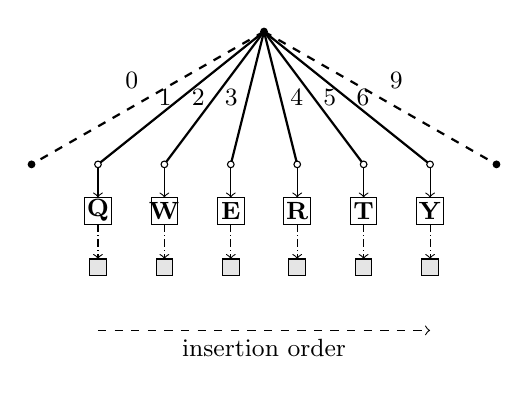
\begin{tikzpicture}[scale=1.2]

  %% node to node
  \small
  \draw[dashed, thick] (0pt,0pt) -- node[anchor=south east]{0} (-70pt,-40pt);
  \draw[thick] (0pt,0pt) -- node[anchor=east]{\DARKBLUE{1}} (-50pt,-40pt);
  \draw[thick] (0pt,0pt) -- node[anchor=east]{\DARKBLUE{2}} (-30pt,-40pt);
  \draw[thick] (0pt,0pt) -- node[anchor=east]{\DARKBLUE{3}} (-10pt,-40pt);
  \draw[thick] (0pt,0pt) -- node[anchor=west]{\DARKBLUE{4}} ( 10pt,-40pt);
  \draw[thick] (0pt,0pt) -- node[anchor=west]{\DARKBLUE{5}} ( 30pt,-40pt);
  \draw[thick] (0pt,0pt) -- node[anchor=west]{\DARKBLUE{6}} ( 50pt,-40pt);
  \draw[dashed, thick] (0pt,0pt) -- node[anchor=south west]{9} ( 70pt,-40pt);

  %% node to element
  \draw[->] (-50pt,-40pt) -- (-50pt,-50pt);
  \draw[->] (-30pt,-40pt) -- (-30pt,-50pt);
  \draw[->] (-10pt,-40pt) -- (-10pt,-50pt);
  \draw[->] ( 10pt,-40pt) -- ( 10pt,-50pt);
  \draw[->] ( 30pt,-40pt) -- ( 30pt,-50pt);
  \draw[->] ( 50pt,-40pt) -- ( 50pt,-50pt);

  %% element to desambiguator
  \draw[->,densely dashdotted] ( -50pt,-58pt) -- ( -50pt,-68.5pt);
  \draw[->,densely dashdotted] ( -30pt,-58pt) -- ( -30pt,-68.5pt);
  \draw[->,densely dashdotted] ( -10pt,-58pt) -- ( -10pt,-68.5pt);
  \draw[->,densely dashdotted] (  10pt,-58pt) -- (  10pt,-68.5pt);
  \draw[->,densely dashdotted] (  30pt,-58pt) -- (  30pt,-68.5pt);
  \draw[->,densely dashdotted] (  50pt,-58pt) -- (  50pt,-68.5pt);

  \draw[fill=black] (  0pt,  0pt) circle (1pt);
  \draw[fill=black] (-70pt,-40pt) circle (1pt);
  \draw[fill=white] (-50pt,-40pt) circle (1pt);
  \draw[fill=white] (-30pt,-40pt) circle (1pt);
  \draw[fill=white] (-10pt,-40pt) circle (1pt);
  \draw[fill=white] ( 10pt,-40pt) circle (1pt);
  \draw[fill=white] ( 30pt,-40pt) circle (1pt);
  \draw[fill=white] ( 50pt,-40pt) circle (1pt);
  \draw[fill=black] ( 70pt,-40pt) circle (1pt);

  %% elements
  \draw[fill=white](-50pt,-54pt)
  node{\textbf{Q}}+(-4pt,-4pt)rectangle+(4pt,4pt) ;
  \draw[fill=white](50pt,-54pt)
  node{\textbf{Y}} +(-4pt,-4pt) rectangle +(4pt,4pt) ;
  \draw[fill=white]( 10pt,-54pt)
  node{\textbf{R}} +(-4pt,-4pt) rectangle +(4pt,4pt) ;
  \draw[fill=white] ( -30pt,-54pt)
  node{\textbf{W}} +(-4pt,-4pt) rectangle +(4pt,4pt) ;
  \draw[fill=white] ( -10pt,-54pt)
  node{\textbf{E}} +(-4pt,-4pt) rectangle +(4pt,4pt) ;
  \draw[fill=white]( 30pt,-54pt)
  node{\textbf{T}} +(-4pt,-4pt) rectangle +(4pt,4pt) ;

  %% desambiguator
  \draw[fill=gray!20] (-50pt,-71pt) +(-2.5pt,-2.5pt) rectangle +(2.5pt,2.5pt);
  \draw[fill=gray!20] (-30pt,-71pt) +(-2.5pt,-2.5pt) rectangle +(2.5pt,2.5pt);
  \draw[fill=gray!20] (-10pt,-71pt) +(-2.5pt,-2.5pt) rectangle +(2.5pt,2.5pt);
  \draw[fill=gray!20] ( 10pt,-71pt) +(-2.5pt,-2.5pt) rectangle +(2.5pt,2.5pt);
  \draw[fill=gray!20] ( 30pt,-71pt) +(-2.5pt,-2.5pt) rectangle +(2.5pt,2.5pt);
  \draw[fill=gray!20] ( 50pt,-71pt) +(-2.5pt,-2.5pt) rectangle +(2.5pt,2.5pt);

  %% insertion order
  \draw[->,dashed] (-50pt, -90pt) -- node[anchor=north]{insertion order}
  (50pt, -90pt);

\end{tikzpicture}
}
    \hspace{20pt}
    \subfloat[Sous-fonction d'allocation conçue pour l'édition de droite à gauche]
    [\label{repl:fig:suballocationB}Sous-fonction d'allocation conçue
    pour l'édition de droite à gauche]
    {\input{input/replication/figsuballocationB.tex}}
    \caption[Deux sous-fonctions d'allocation]
    {\label{repl:fig:suballocation}Deux sous-fonctions d'allocation.}
  \end{center}
\end{figure}

La figure~\ref{repl:fig:suballocation} décrit le fonctionnement des deux
sous-fonctions d'allocation employées par \LSEQ. Les arbres possèdent une arité
maximale de 256 fils à ce niveau. Lorsqu'une insertion est effectuée, un nombre
aléatoire est tiré dans l'espace disponible avec une borne supérieure imposée
(la \emph{boundary}). Cette borne permet de laisser un petit espace libre entre
les identifiants des caractères.% afin de laisser du jeu pour les éventuelles
%corrections orthographiques.
Comme le montre la figure~\ref{repl:fig:suballocationA}, si la borne commence
proche du caractère précédent, alors la fonction d'allocation est adaptée à
l'édition de gauche à droite car elle laisse un espace important pour les
insertions à venir à droite du nouvel élément. Au contraire, comme le montre la
figure~\ref{repl:fig:suballocationB}, si la borne commence proche du caractère
suivant, alors la fonction d'allocation est adaptée à l'édition de droite à
gauche.

\subsection{Choix de sous-fonction d'allocation}
\label{repl:subsec:allocationchoice}

L'utilisation de plusieurs sous-fonctions d'allocation oblige à choisir parmi
celles-ci. Cela pose deux problèmes, à savoir,
\begin{inparaenum}[(i)]
\item quel événement déclenche une prise de décision, et lorsque cela survient, 
\item quelle sous-fonction employer.
\end{inparaenum}

Pour chaque niveau de l'arbre, \LSEQ assigne une sous-fonction d'allocation
grâce à une fonction de hachage. Cette fonction doit retourner les même
résultats quel que soit le participant. Pour cela, une graine, commune à tous
les participants, est placée dans la séquence répliquée. Lorsqu'un nouveau
participant arrive, il réplique la graine avec la séquence.

Afin de ne privilégier aucun comportement d'édition, le choix parmi les
sous-fonctions doit être uniformément réparti. De plus, afin de ne pas faciliter
les comportements malveillants, la fonction de hachage doit rendre les choix
imprévisibles.

\subsection{Conclusion}

\begin{figure}
  \begin{center}
    \subfloat[Édition de gauche à droite dans \LSEQ]
    [\label{repl:fig:lseqtreeexampleA} Édition de gauche à droite dans \LSEQ]
    {\input{input/replication/figlseqtreeexampleA.tex}}
    \subfloat[Édition de droite à gauche dans \LSEQ]
    [\label{repl:fig:lseqtreeexampleB} Édition de droite à gauche dans \LSEQ]
    {\input{input/replication/figlseqtreeexampleB.tex}}
    \caption[Gestion des comportements d'édition par \LSEQ]
    {\label{repl:fig:lseqtreeexample} Exemple d'arbres exponentiels \LSEQ
      remplis par deux comportements d'édition antagonistes résultant sur une
      même séquence \texttt{QWERTY}.}
  \end{center}
\end{figure}

L'idée générale de \LSEQ consiste à accepter la perte de niveaux des chemins
composants ses identifiants pour peu que les futures allocations compensent ces
pertes.


La figure~\ref{repl:fig:lseqtreeexample} montre le résultat de la stratégie
d'allocation \LSEQ après deux comportements d'éditions : l'un écrit de gauche à
droite, l'autre écrit de droite à gauche. Dans les deux cas, la séquence est
\texttt{QWERTY}; l'arité maximale commence à $2^5$ et est doublée à chaque
niveau; la fonction de hachage désigne comme étant les sous-fonctions conçues
pour l'édition de gauche à droite, et pour l'édition de droite à gauche, pour
les niveaux 1 et 2 respectivement. La figure~\ref{repl:fig:lseqtreeexampleA}
montre le cas de l'édition de gauche à droite. Dans ce cas, le comportement
d'édition attendu par la sous-fonction d'allocation est bon, et les chemins
restent alloués au premier niveau de l'arbre. D'un autre coté, la
figure~\ref{repl:fig:lseqtreeexampleB} montre le cas de l'édition de droite à
gauche. Dans ce cas, la sous-fonction d'allocation du premier niveau n'est pas
adaptée. La profondeur de l'arbre augmente dès la seconde insertion. En
revanche, puisque la sous-fonction d'allocation choisie à ce niveau est adaptée,
la profondeur de l'arbre n'augmente pas d'avantage. Si le comportement d'édition
reste ainsi, l'allocation finira par compenser les pertes subies par le mauvais
choix de sous-fonction au premier niveau de l'arbre. 

La section suivante présente l'analyse en complexité de \LSEQ. En particulier,
elle s'attache à montrer la complexité spatiale sous-linéaire des identifiants
ainsi que les conditions sous lesquelles elle s'applique.

%%% Local Variables:
%%% mode: latex
%%% TeX-master: "../../paper"
%%% End:
